\section{Løsninger til linære programmeringsproblemer}

Den mulige mængde er mængden af løsningsvektorer, $\vec{x}$, som opfylder alle problemets betingelser. Hvis en optimal løsning eksisterer, vil denne derved være indeholdt i den mulige mængde.

\begin{defn}[Mulige løsninger og den mulige mængde]
En \textbf{mulig løsning} er en løsningsvektor $\vec{x}$, som opfylder alle problemets betingelser.\\
\textbf{Den mulige mængde} $\mathcal{F}$ er mængden af alle de mulige løsninger. Den vil derfor, for et standard maksimeringsproblem, være defineret som
\begin{align*}
\mathcal{F}=\{\vec{x} \in \mathds{R}^n|A\vec{x} \leq \vec{b}, \vec{x} \geq \vec{0}\}.
\end{align*}
Et problem kaldes \textbf{inkonsistent}  hvis den mulige mængde er den tomme mængde, ellers er problemet \textbf{konsistent}. 
\end{defn}

I lineær programmering søges der efter en optimal løsning, som vil være den mulige løsning, der enten maksimerer eller minimerer objektfunktionen, afhængig af, om der er tale om et maksimerings- eller minimeringsproblem. 
Husk på, at et maksimeringsproblem kan laves til et minimeringsproblem, hvorfor det kun er nødvendigt at definere den optimale løsningsværdi for minimeringsproblemet.
\begin{defn}[Optimal løsningsværdi]
Lad $f$ være objektfunktionen til et lineært minimeringsproblem, da kaldes en vektor $\vec{x}^*$ en \textbf{optimal løsningsværdi}, hvis 
\begin{align}
	f(\vec{x}^*)=\min\limits_{\vec{x} \in \mathcal{F}}f(\vec{x}).
\end{align}
Værdien af $f(\vec{x}^*)$ kaldes den \textbf{optimale værdi}.
\end{defn}

Den optimale løsning kan findes på forskellige måder, heriblandt med Simplex metoden, som beskrives i Kapitel \ref{chap:simp}. En anden måde er ved geometrisk visualisering af den mulige mængde. Denne metode er mulig for problemer med op til 3 variable, da løsningsmængden derved visualiseres som et plot i det tilsvarende antal dimensioner. De mulige løsninger findes således inden for det område, der er begrænset af betingelserne. 

\begin{eks}[Den mulige mængde]
Ved at indtegne betingelserne i et koordinatsystem er det muligt at visualisere den mulige mængde som fællesmængden af de mængder, der dannes ud fra betingelserne. På Figur \ref{fig:maksprob2} er den mulige mængde for problemet i Eksempel \ref{eks:maksprob2} indtegnet. Der er desuden tegnet en pil for hver betingelse, som viser, for hvilken side af linjen, koordinaterne opfylder betingelsen. Den mulige mængde er farvet grå.

\begin{center}
	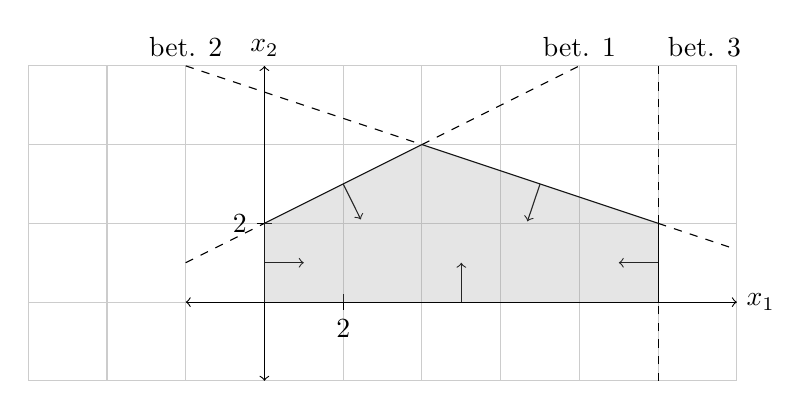
\begin{tikzpicture}
  %laver Grid. godt til når koordinater skal redigeres
  	\draw[thin,gray!40] (-3,-1) grid (6,3); 
  %x-aksen
  	\draw[<->] (-1,0)--(6,0) node[right]{$x_1$};
  	\draw[->] (2.5,0) -- (2.5,0.5);
  %y-aksen
  	\draw[<->] (0,-1)--(0,3) node[above]{$x_2$};
  	\draw[->] (0,0.5) -- (0.5,0.5);
  	
  %akse-markeringer
  	%\node[left] (xakse) at (0,1) {2};
  	\draw[] (-0.1,1) -- (0.1,1) node[pos=0,left] {2};
  	\draw[] (1,-0.1) -- (1,0.1) node[pos=0,below] {2};
  	
  %ligning 1
	\draw[domain=-1:0,variable=\x,dashed] 	plot({\x},{0.5*\x+1});
	\draw[domain=0:2,variable=\x] 			plot({\x},{0.5*\x+1});
	\draw[domain=2:4,variable=\x,dashed] 	plot({\x},{0.5*\x+1}) node[above] {bet. 1};
  	\draw[->] (1,1.5) -- (1.224,1.05);
	
  %ligning 2
  	\draw[domain=-1:2,variable=\x,dashed] 	plot({\x},{-(1/3)*\x+8/3}) node[above] at (-1,3) {bet. 2} ;
	\draw[domain=2:5,variable=\x] 			plot({\x},{-(1/3)*\x+8/3});
	\draw[domain=5:6,variable=\x,dashed] 	plot({\x},{-(1/3)*\x+8/3});
	\draw[->] (3.5,1.5) -- (3.34,1.026);

  %ligning 3
  	\draw[domain=-1:0,variable=\y,dashed] 	plot({5},{\y});
	\draw[domain=0:1,variable=\y] 			plot({5},{\y});
	\draw[domain=1:3,variable=\y,dashed] 	plot({5},{\y}) node[above right] {bet. 3};
	\draw[->] (5,0.5) -- (4.5,0.5);

  %løsningsmængden skraveret
	\fill[gray!80,nearly transparent] (0,0) -- (0,1) -- (2,2) -- (5,1) --(5,0) --  cycle;
\end{tikzpicture}
	\captionof{figure}{Skravering af den mulige mængde for et standard maksimeringsproblem.}
	\label{fig:maksprob2}
\end{center}
\end{eks}

Løsningerne til et optimeringsproblem er beskrevet som værende alle de vektorer, $\vec{x}$, som overholder bibetingelserne. Løsningsmængden til bibetingelserne er beskrevet som et polyeder.
\begin{defn} [Polyeder]
Et \textbf{Polyeder} er en mængde 
\begin{align*}
 P =\{ \vec{x} \in \mathds{R}^n | A \vec{x} \geq \vec{b}, \vec{b}\in \mathds{R}^m\},
\end{align*}
hvor $A$ er en $m \times n$ matrix.
\end{defn}
Hvis et lineært programmeringsproblem står på standardform med ligheder $\{ \vec{x} \in \mathds{R}^n | A \vec{x} = \vec{b}, \vec{b}\in \mathds{R}^m\}$, så kaldes det stadig et polyeder.\\
Hvis der er et polyeder $P=\{\vec{x} \in \mathds{R}\mid A\vec{x}=\vec{b},\vec{x}\geq \vec{0}\}$, som består af alle bibetingelserne for problemet, så må der også findes et andet polyeder $Q$, som består af alle de lineært uafhængige bibetingelser for problemet. Da $P$ består af de samme bibetingelser som $Q$ og lidt flere til, så er en løsning $\vec{x}$ til $P$ nødvendigvis også en løsning til $Q$, og modsat er en løsning til $Q$ også en løsning til $P$. Derfor må $Q=P$, hvilket vil blive vist i følgende sætning.

\begin{stn}[Q=P]
Lad $P=\{\vec{x} \in \mathds{R}^n\mid A\vec{x}=\vec{b},\vec{x}\geq \vec{0}\}$ være et ikke-tomt polyeder, hvor $A$ er en $m\times n$ matrix.\\
Antag at $rang(A)=k<m$ og at rækkerne $\vec{a_i}^T$ for $i=1,\dots ,k$ er lineært uafhængig. Betragt polyederet $Q=\{\vec{x} \in \mathds{R}^n\mid \vec{a_i}^T\vec{x}=b_{i}, \vec{x}\geq \vec{0}, i = 1,\dots	k\}$. Så er $Q=P$.
\label{stn:PQ}
\end{stn}

\begin{proof}
Hvis $P=\{\vec{x} \in \mathds{R}^n\mid A\vec{x}=\vec{b}, \vec{x}\geq \vec{0}\}$ er et polyeder med $rang(A)=k$, afgrænset af alle bibetingelserne, så må der være et polyeder $Q=\{\vec{x} \in \mathds{R}^n\mid \vec{a_i}^T\vec{x}=b_{i}, \vec{x}\geq \vec{0}, i = 1,\dots,	k\}$, der består af alle lineært uafhængige bibetingelser. Så må $P\subseteq Q$, eftersom alle elementerne i $P$ også tilfredsstiller bibetingelserne for $Q$.\\
Eftersom $rang(A)=k$, så former rækkerne $\vec{a_1},\dots ,\vec{a_k}$ en basis for rækkerummet. Derfor kan enhver række $\vec{a}_j$ fra $A$ skrives som en linearkombination af de lineært uafhængige rækker $\vec{a}_i$ for $i = 1,...,k$.
Dermed bliver $\vec{a}_j = \sum_{i=1}^k c_{ij}\vec{a}_i$ for skalarer $c_{ij}$.

 Lad så $\vec{x}$ være en del af $P$ så
\begin{align*}
\vec{a}_j^T\vec{x}=\sum_{i=1}^{k}c_{i j}\vec{a}_i^T\vec{x}=\sum_{i=1}^{k}c_{i j}\vec{b}_i=\vec{b}_j, \qquad j=1,\dots,m.
\end{align*}
Derfor kan det konkluderes, at $P \subseteq Q$.\\
Lad nu $\vec{y}$ være en del af $Q$, så er $\vec{y}$ også en del af $P$, eftersom
\begin{align*}
\vec{a}_j^T\vec{y}=\sum_{i=1}^{k}c_{i j}\vec{a}_i^T\vec{y}=\sum_{i=1}^{k}c_{i j}\vec{b}_i=\vec{b}_j, \qquad j=1,\dots,m.
\end{align*}
Hvilket betyder, at $\vec{y}\in P$ og $Q\subseteq P$, og derved er $P=Q$.
\end{proof}

Derfor kan det antages, at alle bibetingelserne er lineært uafhængige uden at miste generelitet. 

%Et polyeder kan, alt efter bibetingelserne, være en mængde, der strækker sig ud i det uendelige, eller det kan være begrænset. 
%Hvis der er med et maksimeringsproblem at gøre, kan det ses, at bibetingelserne danner et område, men ved et minimeringsproblem, vil bibetingelserne ofte resultere i, at polyederet strækker sig ud i det uendelige, og derfor ikke længere er en form. Selvom dette er tilfældet, kaldes løsningsmængden stadig for et polyeder. \\
%Et problem kaldes \textbf{ubegrænset}, hvis objektfunktionen kan tage arbitrært store funktionsværdier for maksimeringsproblemer, og arbitrært små funktionsværdier for minimeringsproblemer. Ellers kaldes problemet \textbf{begrænset}.

%\begin{defn} [Begrænset]
%Lad $S \subset \mathds{R}^n$, da er $S$ begrænset, hvis der eksisterer en konstant $K$ så $\forall \vec{x} \in S: |\vec{x}| \leq K$.
%\end{defn}
%
%Med andre ord; hvis der findes en konstant, som er højere end den absolutte værdi af alle $\vec{x} \in S \in S$, og hvis der ikke eksisterer en konstant, som er støre end $|\vec{x}|$, så vil alle $\vec{x}$ gå mod uendeligt.